\section{Конструкторская часть}

В этом разделе будут представлены схемы реализуемых алгоритмов.

<<<<<<< HEAD
=======
<<<<<<< HEAD
<<<<<<< HEAD
=======
Оптимизация алгоритма Винограда заключается:
\begin{itemize}
	\item в замене операций x = x + k на x += k;
	\item в замене умножения на 2 на побитовый сдвиг;
	\item в предвычислении некоторых слагаемых.
\end{itemize}

Для сокращения времени чтения отчёта схема оптимизированного алгоритма не представлена.

>>>>>>> 7ad89dc (lab_02 almost passed)
=======
>>>>>>> af69c2c (lab_02 passed)
>>>>>>> fb5d8bb (lab_02 passed)
\newpage

\subsection{Классический алгоритм перемножения матриц}

Схема классического алгоритма перемножения матриц представлена на рисунке \ref{fig:classic}.
\begin{figure}
	\centering
	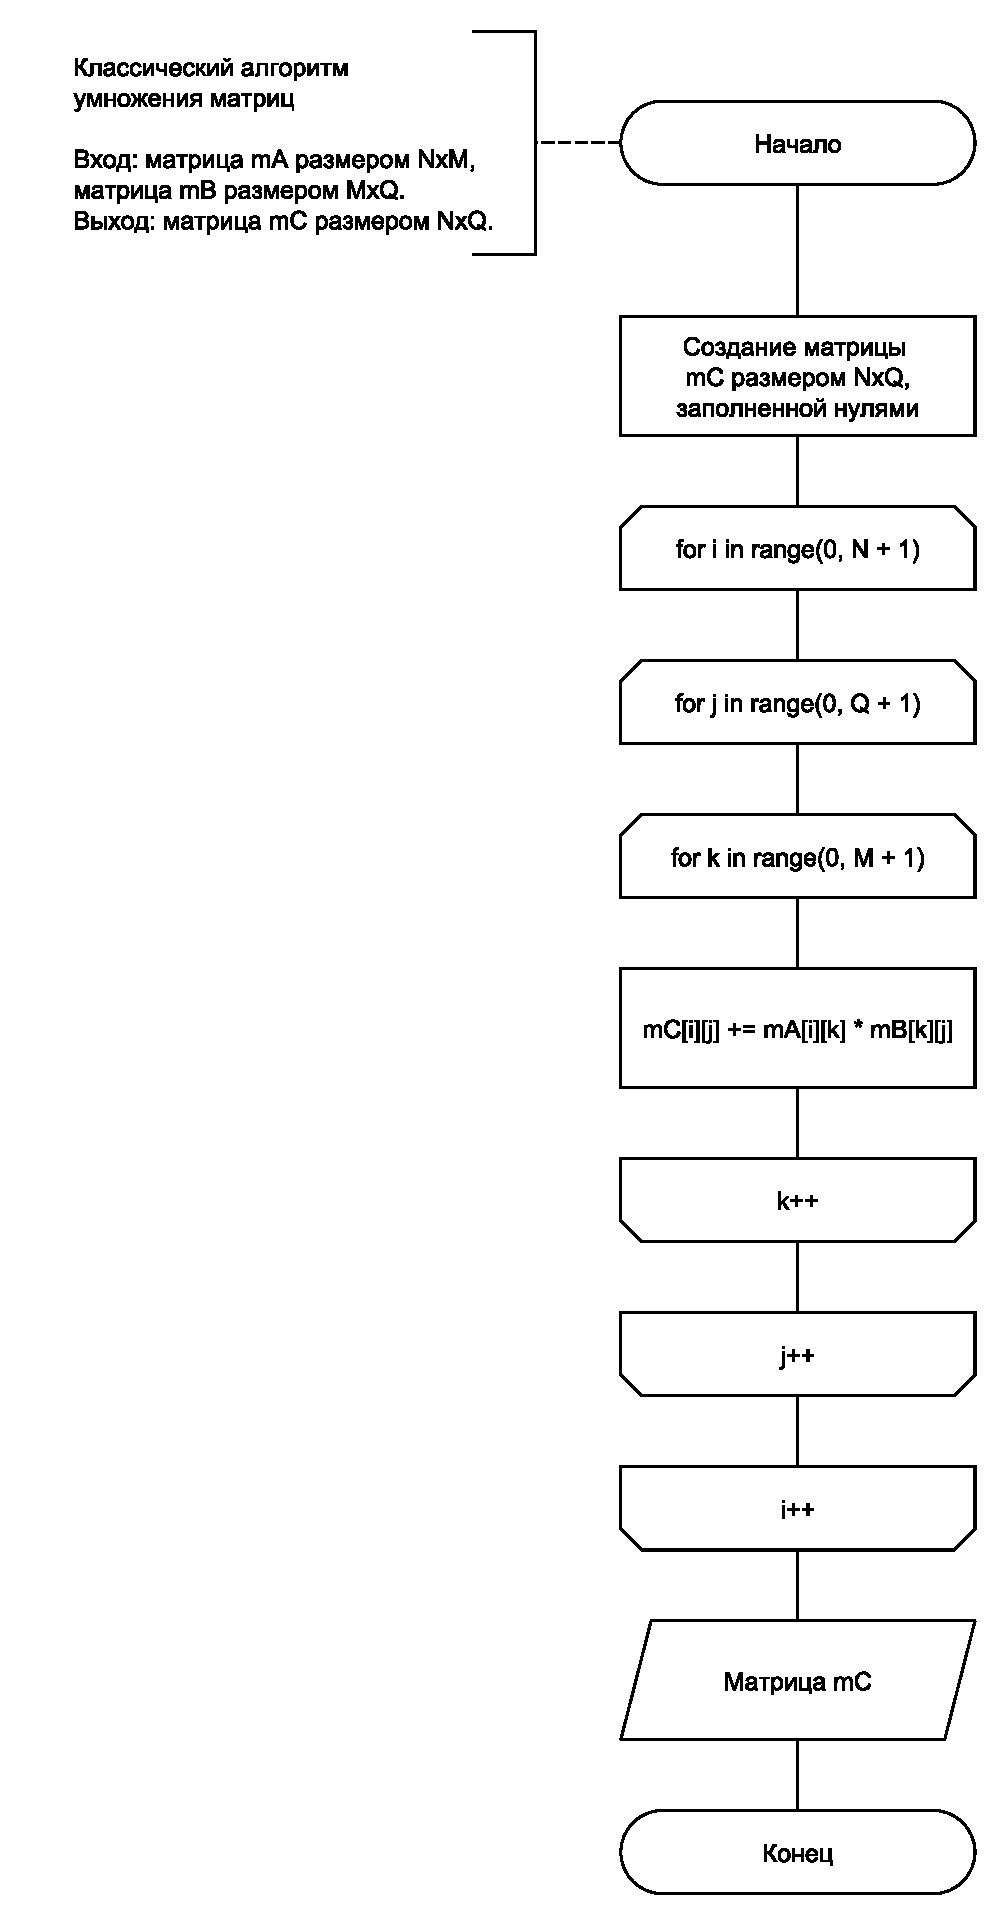
\includegraphics[width=0.6\linewidth]{images/classic}
	\caption{Схема классического алгоритма перемножения матриц}
	\label{fig:classic}
\end{figure}

\newpage

\subsection{Алгоритм Винограда перемножения матриц}

Схема алгоритма Винограда перемножения матриц представлена на рисунке \ref{fig:winograd1} и \ref{fig:winograd2}.

\begin{figure}
	\centering
	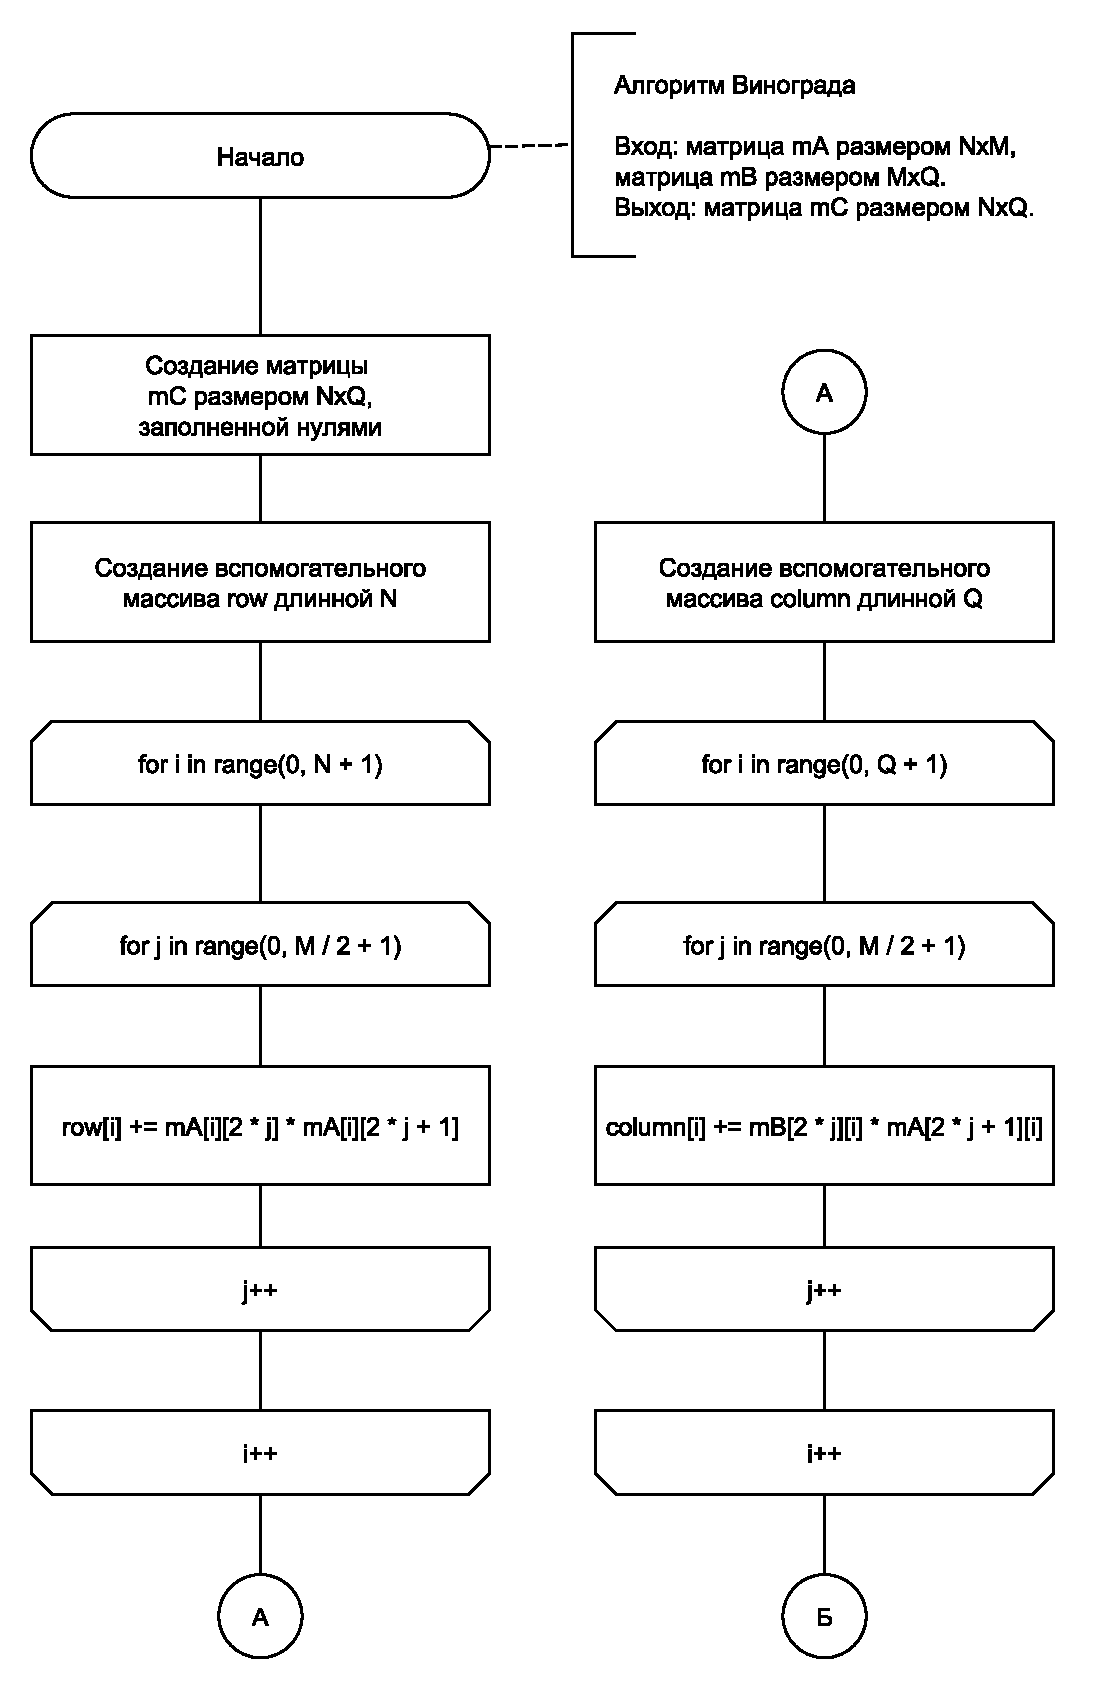
\includegraphics[width=0.75\linewidth]{images/winograd1}
	\caption{Схема алгоритма Винограда}
	\label{fig:winograd1}
\end{figure}

\newpage

\begin{figure}
	\centering
	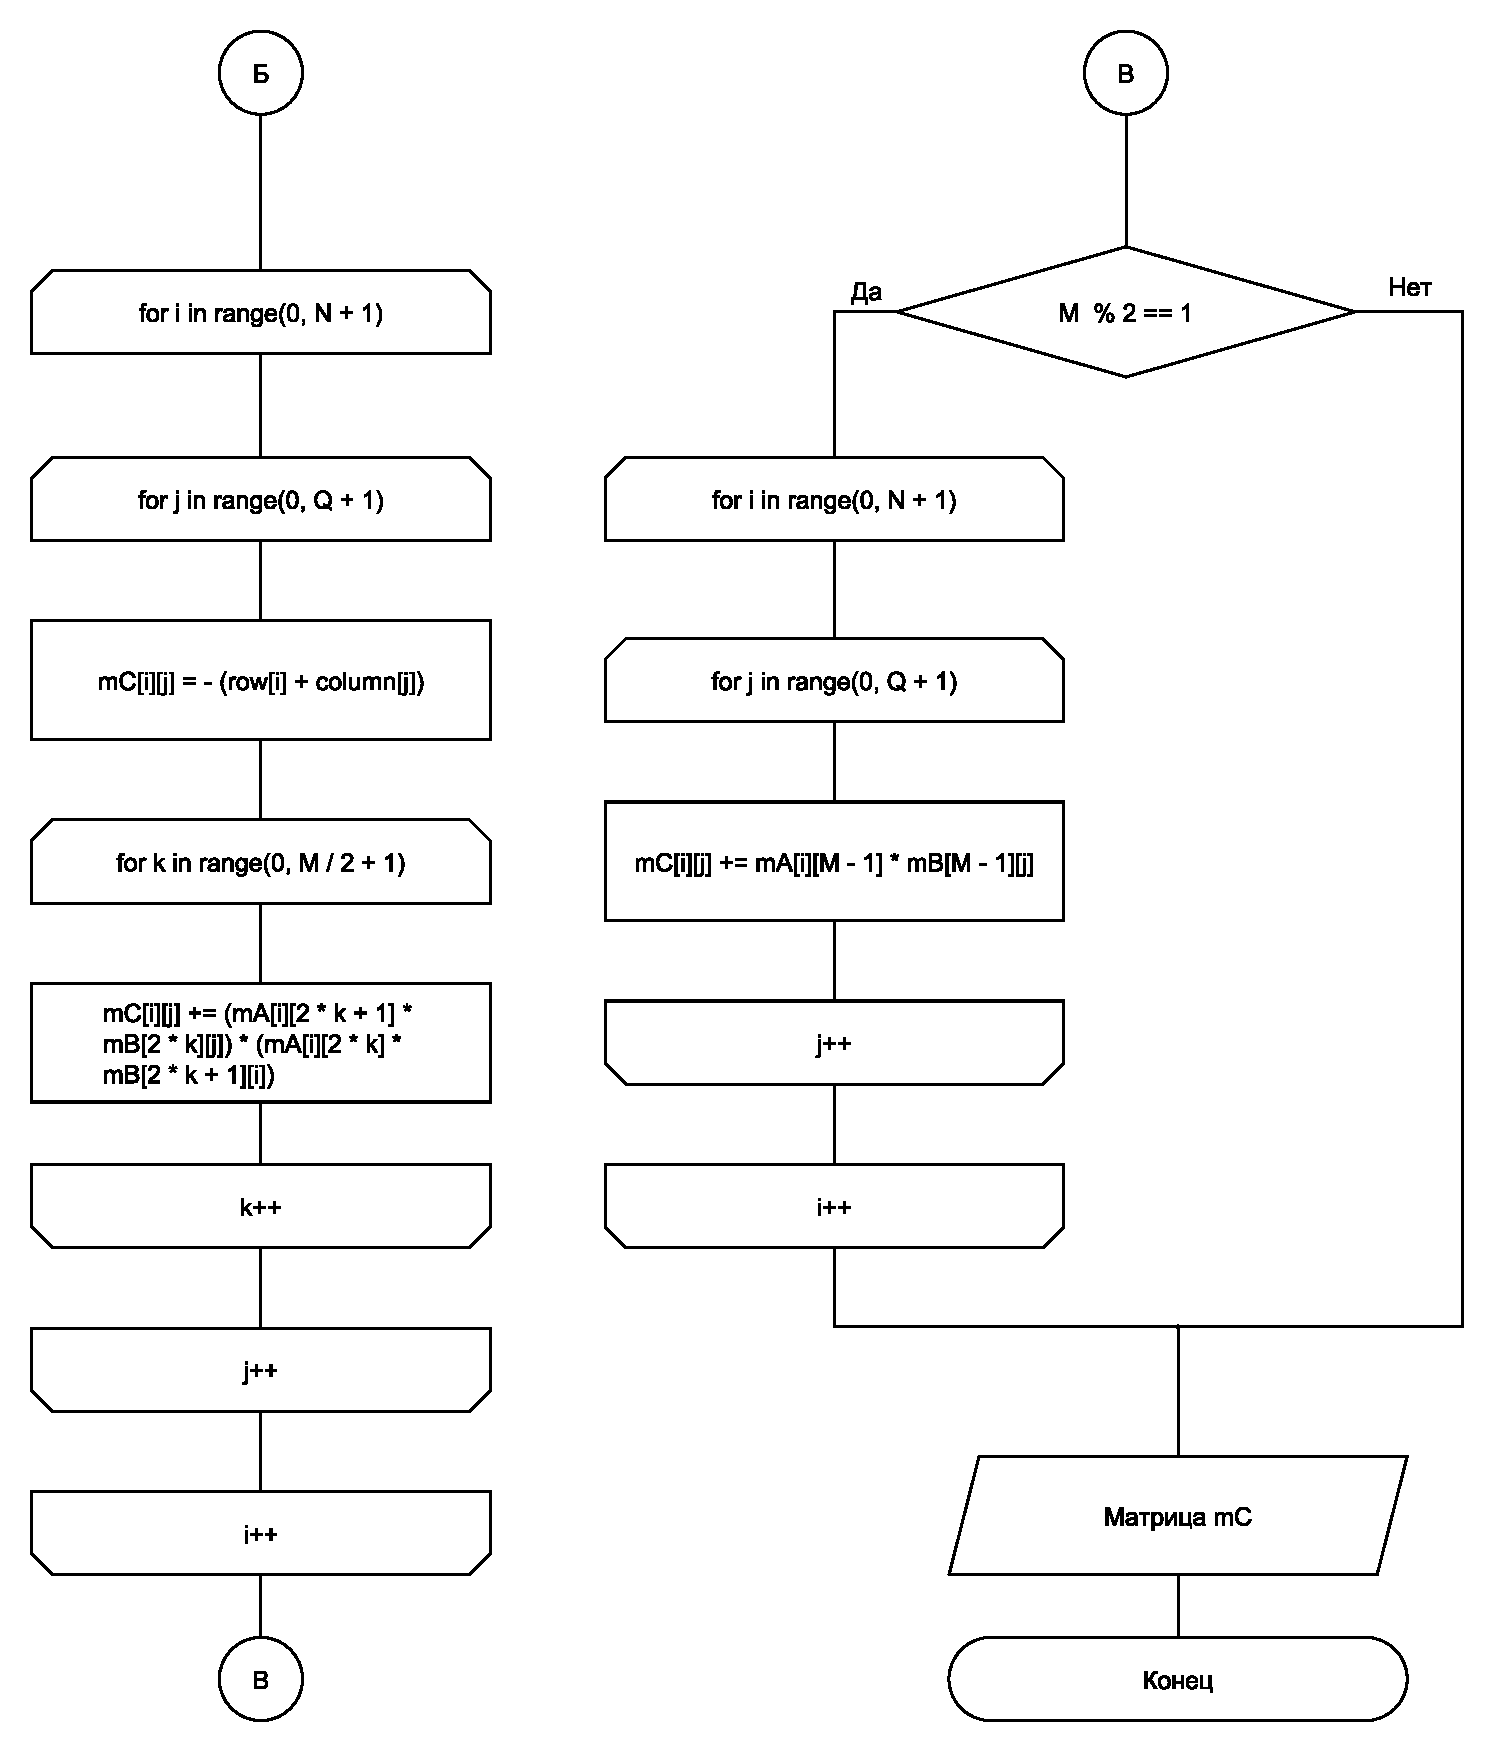
\includegraphics[width=0.9\linewidth]{images/winograd2}
	\caption{Схема алгоритма Винограда (продолжение)}
	\label{fig:winograd2}
\end{figure}

<<<<<<< HEAD
=======
<<<<<<< HEAD
<<<<<<< HEAD
=======
>>>>>>> af69c2c (lab_02 passed)
>>>>>>> fb5d8bb (lab_02 passed)
Оптимизация алгоритма Винограда заключается:
\begin{itemize}
	\item в замене операций x = x + k на x += k;
	\item в замене умножения на 2 на побитовый сдвиг;
	\item в предвычислении некоторых слагаемых.
\end{itemize}

Для сокращения времени чтения отчёта схема оптимизированного алгоритма не представлена.

<<<<<<< HEAD
=======
<<<<<<< HEAD
=======
>>>>>>> 7ad89dc (lab_02 almost passed)
=======
>>>>>>> af69c2c (lab_02 passed)
>>>>>>> fb5d8bb (lab_02 passed)
\newpage

\subsection{Алгоритм Штрассена перемножения матриц}

Схема алгоритма Штрассена перемножения матриц представлена на рисунке \ref{fig:strassen}.

\begin{figure}
	\centering
	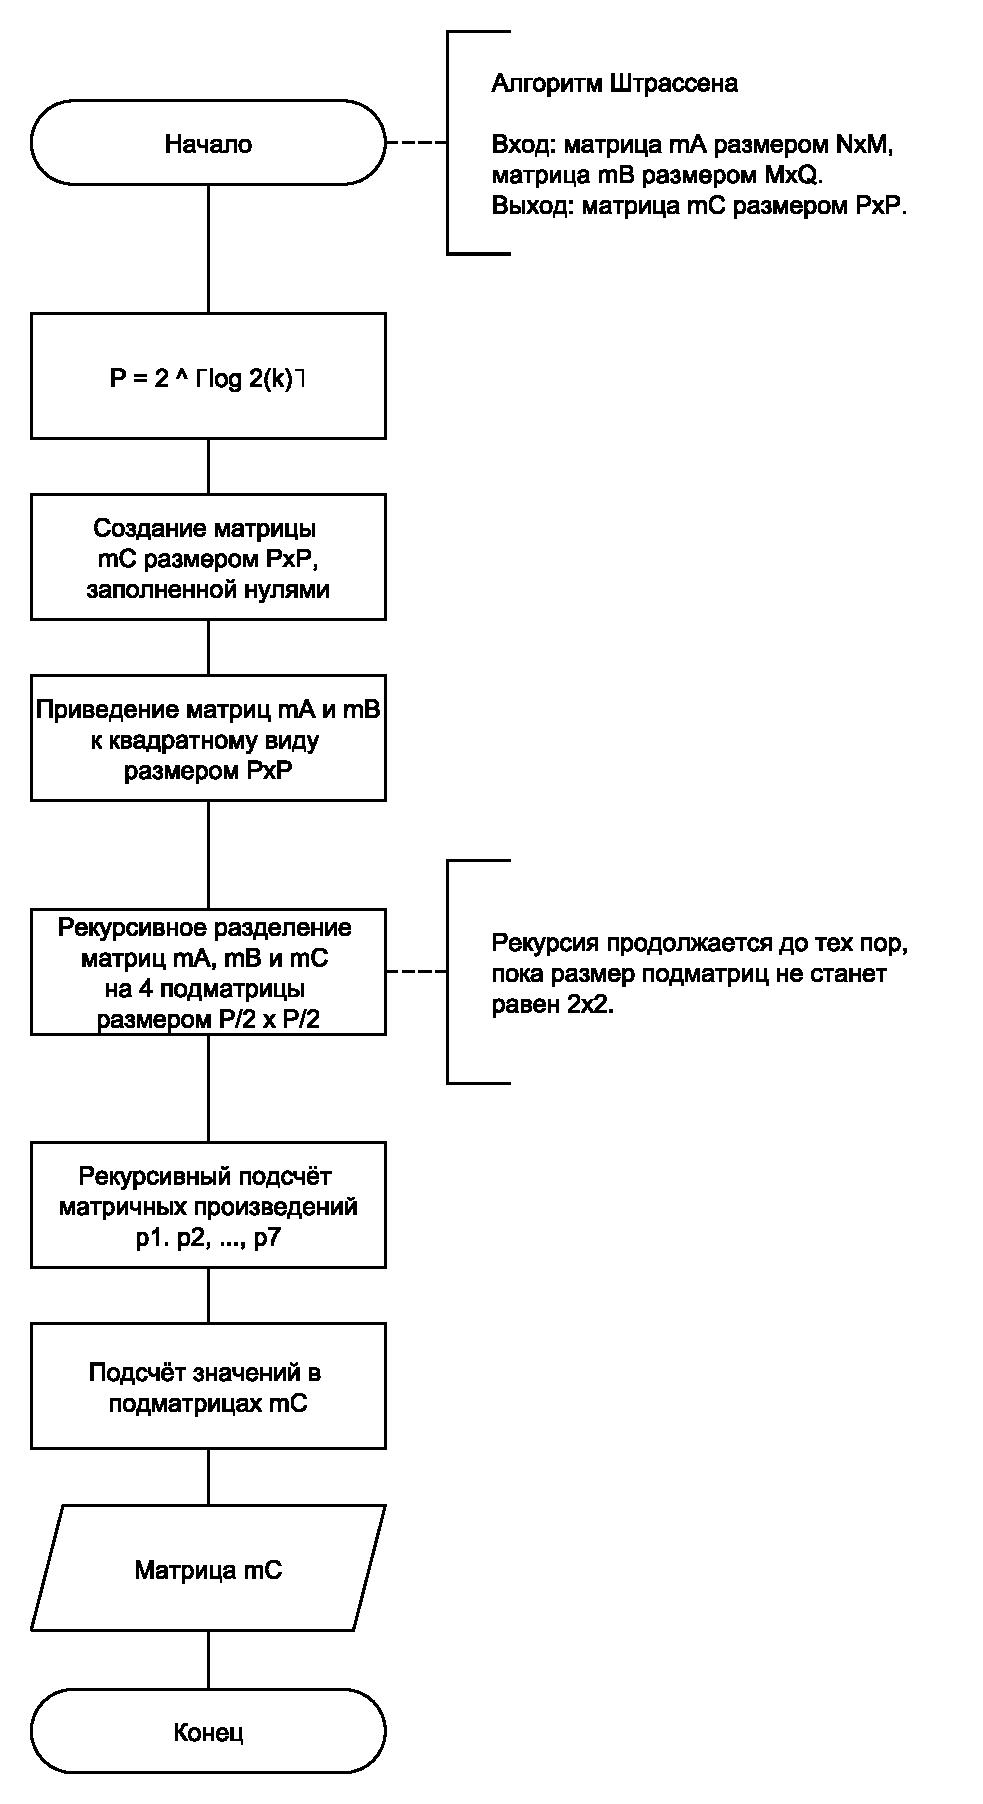
\includegraphics[width=0.65\linewidth]{images/strassen}
	\caption{Алгоритм Штрассена}
	\label{fig:strassen}
\end{figure}

\newpage

\subsection{Модель вычислений}
Для последующего вычисления трудоемкости необходимо ввести модель вычислений:
\begin{enumerate}
	\item операции из списка (\ref{for:opers}) имеют трудоемкость 1;
	\begin{equation}
		\label{for:opers}
		+, -, *, /, \%, ==, !=, <, >, <=, >=, [], ++, {-}-
	\end{equation}
	\item трудоемкость оператора выбора \code{if условие then A else B} рассчитывается как (\ref{for:if});
	\begin{equation}
		\label{for:if}
		f_{if} = f_{\text{условия}} +
		\begin{cases}
			f_A, & \text{если условие выполняется,}\\
			f_B, & \text{иначе.}
		\end{cases}
	\end{equation}
	\item трудоемкость цикла рассчитывается как (\ref{for:for});
	\begin{equation}
		\label{for:for}
		f_{for} = f_{\text{инициализации}} + f_{\text{сравнения}} + N(f_{\text{тела}} + f_{\text{инкремента}} + f_{\text{сравнения}})
	\end{equation}
	\item трудоемкость вызова функции равна 0.
\end{enumerate}


\subsection{Трудоемкость алгоритмов}

В следующих частях будут рассчитаны трудоемкости представленных ранее классического алгоритма и алгоритма Винограда.
Трудоёмкость алгоритма Штрассена в отчёте не приведена, поскольку на занятиях не были рассказаны методы рассчёта трудоёмкости рекурсивных функций.
Трудоёмкость инициализации результирующей матрицы учитываться не будет, поскольку данное действие есть во всех алгоритмах и не является самым трудоёмким.

Введём обозначения:
\begin{itemize}
	\item N -- кол-во строк первой матрицы;
	\item M -- кол-во столбцов первой матрицы и кол-во строк второй матрицы;
	\item Q -- кол-во столбцов второй матрицы.
	
\end{itemize}

<<<<<<< HEAD
\newpage
=======
<<<<<<< HEAD
<<<<<<< HEAD
\newpage
=======
>>>>>>> 7ad89dc (lab_02 almost passed)
=======
\newpage
>>>>>>> af69c2c (lab_02 passed)
>>>>>>> fb5d8bb (lab_02 passed)
\subsubsection{Классический алгоритм перемножения матриц}

Трудоёмкость стандартного алгоритма умножения матриц состоит из:

\begin{itemize}
	\item внешнего цикла по $i \in [1..M]$, трудоёмкость которого: $f = 2 + M \cdot (2 + f_{body})$;
	\item цикла по $j \in [1..N]$, трудоёмкость которого: $f = 2 + N \cdot (2 + f_{body})$;
	\item цикла по $k \in [1..Q]$, трудоёмкость которого: $f = 2 + 10 \cdot Q$.
\end{itemize}

Трудоёмкость классического алгоритма равна трудоёмкости внешнего цикла.
Её можно вычислить, подставив циклы тела (\ref{for:classic}):
\begin{equation}
	\label{for:classic}
	f_{classic} = 2 + M \cdot (4 + N \cdot (4 + 10Q)) = 2 + 4M + 4MN + 10MQN \approx 10MQN
\end{equation}

\subsection{Алгоритм Винограда}

Трудоёмкость алгоритма Винограда состоит из:
\begin{itemize}
	\item создания и инициализации массивов row и column, трудоёмкость которого (\ref{for:init}):
	\begin{equation}
		\label{for:init}
		f_{init} = N + Q;
	\end{equation}
	
	\item заполнения массива row, трудоёмкость которого (\ref{for:row}):
	\begin{equation}
		\label{for:row}
		f_{row} = 2 + N \cdot (2 + \frac{M}{2} \cdot 11);
	\end{equation}
	
	\item заполнения массива column, трудоёмкость которого (\ref{for:column}):
	\begin{equation}
		\label{for:column}
		f_{column} = 2 + Q \cdot (2 + \frac{M}{2} \cdot 11);
	\end{equation}
	
	\item цикла заполнения для чётных размеров, трудоёмкость которого (\ref{for:cycle}):
	\begin{equation}
		\label{for:cycle}
		f_{cycle} = 2 + N \cdot (2 + Q \cdot (23 \cdot \frac{M}{2}));		
	\end{equation}
	
	\item цикла, для дополнения результирующего массива суммой последних нечётных строки и столбца, если общий размер нечётный, трудоемкость которого (\ref{for:last}):
	\begin{equation}
		\label{for:last}
		f_{last} = \begin{cases}
			2, & \text{размер чётный,}\\
			2 + N \cdot (2 + 14Q), & \text{иначе.}
		\end{cases}
	\end{equation}
\end{itemize}

%(N + Q) + (2 + 2N + 11/2*MN) + (2 + 2Q + 11/2*MQ) + (2 + 2N + 23/2*MNQ) + (2 или 2 + 2N + 14NQ) 
%= 2 + 2 + 2 + N + 2N + 2N + Q + 2Q + 5.5MN + 5.5MQ + 11.5MNQ + (2 или 2 + 2N + 14NQ) 
%= 6 + 5N +3Q + 5.5MN + 5.5MQ + 11.5MNQ + (2 или 2 + 2N + 14NQ)

% 6 + 5N + 3Q + 5.5M(N + Q) + 11.5MNQ +
%\begin{cases}
%	2, & \text{размер чётный,}\\
%	2 + 2N + 14NQ, & \text{иначе.}
%\end{cases} 

Итого, результирующая трудоёмкость алгоритма Винограда равна (\ref{for:final})
\begin{equation}
	\label{for:final}
	f_{final} = f_{row} + f_{column} + f_{cycle} + f_{last} \approx 11.5MNQ
\end{equation}